\chapter[Statistical Treatment][Statistical Treatment]{Statistical Treatment}
\label{app:statisticaltreatment}

The underlying statistical measure used in this analysis for comparing the goodness of fit of a statistical model to data is the \emph{likelihood function}, a joint probability distribution of the sample viewed as a function of the parameters only.
According to the likelihood principle proposition, the likelihood function contains all the evidence in a sample relevant to model parameters, given a statistical model.
Constructing this likelihood function will thereby result in the full statistical model to be tested for this analysis.

\section{The Likelihood Function}
For experiments with a large number of independent discrete events, such as ATLAS, a Poisson distribution, $P(k;\lambda)$, is the valid probability distribution.
Where $k$ is the number of observed events and $\lambda$ the expectation of the given model.
Each analysis region included in the analysis will have a corresponding independent Poisson that forms the likelihood function.
Regions included are the signal regions, \SRTL, \SRFour, and \SRThree of which are further subdivided into bins of \mZl, the primary discriminating variable discussed in Section \ref{sec:strategy:signal}, in order to maximize the discovery sensitivity to a resonance. 
The binning of the \mZl observable was optimized using simulated \CCsignal and \CNsignal signal samples with reconstructed mass resolutions of around 2\%, and the optimized binning accounts for the predicted background expectation.
Lower edges are set to
\begin{equation}
  m_{Z\ell} = 90, 110, 130, 150, 170, 190, 210, 230, 250, 270, 300, 330, 360, 400, 440, \mathrm{~and~}580~GeV.
  \label{eq:binning}
\end{equation}
The last bin has no upper edge and includes all events with \mZl\ $>$ 580~\GeV.
The same binning is used for all three SRs, facilitating the discovery of a trilepton resonance that would contribute to all SRs.
This effectively results in (3SRs$\times 16 $~\mZl bins) = 48 independent signal regions.
The three control regions, \CRWZ, \CRttZ, and \CRZZ are also included in the fit to better estimate the corresponding major backgrounds.
The systematic uncertainties' probability distributions are modeled as Gaussians, $g(\boldsymbol\theta_{0}, \boldsymbol\theta)$, who's means and widths are determined by dedicated auxiliary measurements, $\boldsymbol\theta_{0}$, collected by ATLAS performance groups.
The full statistical model is then written down as the Likelihood in Equation \ref{eq:statmodel}.
\begin{equation}
\begin{split}
    \mathcal{L}(\boldsymbol\theta|k)=\prod_{i}\frac{\lambda_{i}^{k_{i}}e^{-\lambda_{i}}}{k_{i}!}\times \prod_{systs}g(\boldsymbol\theta_{0},\boldsymbol\theta)& , \qquad
    \lambda_{i} = \mu_{sig} s_{i}(\boldsymbol\theta)+b_{i}(\boldsymbol\theta) \\
    i = \textrm{CR}t\bar{t}Z,\textrm{CR}WZ,\textrm{CR}ZZ, &SR_{0}, SR_{1},..., SR_{48}  \\
    \boldsymbol\theta = (\mu_{ttZ},\mu_{WZ},\mu_{ZZ}&, NP_{0}, NP_{1}, ...)
\end{split}
\label{eq:statmodel}
\end{equation}
Where $\boldsymbol\theta$ is the set of two types of parameters that will be allowed to float in the ultimate fit to the data.
The first type are the \emph{normalization factors}, derived from the yields of the three main background contributors \ttZ, \WZ, and \ZZ.
And while the \ttZ, \WZ, and \ZZ yields are allowed to float in all regions in the fit the values of $\mu_{ttZ},\mu_{WZ},$ and $\mu_{ZZ}$ will be determined by and large by the high purity/stats the dedicated control regions give us. 
The second type are known as \emph{nuisance parameters}, and are degrees of freedom corresponding to the suite of systematic uncertainties included in the analysis and are constrained by their corresponding Gaussians.
$i$ is then the group of analysis regions to be fit simultaneously, the details of which is to be discussed in Sections~\ref{sec:stats:bkgonly} to ~\ref{sec:stats:moddep}.
%If there are two fully leptonic \Zl pairs, the average of both is taken because the mass resolution of each should be similar.
%The masses of each are also guaranteed to be similar because of the \MZlAsym$<$ 0.1 requirement in \SRTL (described in \ref{sec:srfr}).
%This shape fit uses a variable bin width in the \mZl distribution, optimized through the full \Histfitter machinery.
Three types of fits are required in order to both validate background estimations and to make model dependent and model independent physics statements and are detailed in Sections~\ref{sec:stats:bkgonly} to ~\ref{sec:stats:moddep}. 

\section{Goodness of Fit: Maximum Likelihood Estimation}
\label{sec:stats:MLE}
The goodness of fit measure used is the powerful Maximum Likelihood Estimate (MLE), which is the method of estimating parameters of a probability distribution by maximizing it's likelihood function so that under the assumed statistical model the observed data is most probable.

\subsection{The Profile Likelihood}
\label{sec:stats:ProfileLiklihood}
In physics analyses such as these, which many parameters must be estimated, reducing the parameters to only the parameters of interest by eliminating nuisance parameters becomes effectively essential in order to have a tractable problem.
This is done via the procedure known as the \emph{profile likelihood}.
This amounts to concentrating the likelihood function for a subset of parameters by expressing the nuisance parameters as functions of the parameters of interest and then replacing them in the likelihood function.
In this case a single parameter, $\mu_{sig}$, the signal strength parameter, is the parameter of interest.
Graphically the profile likelihood can be seen as a ridge for which the likelihood is maximized for values of $\mu_{sig}$, with the maximum likelihood estimator then taking on $\boldsymbol\theta=\hat{\vphantom{\rule{1pt}{0.1ex}}\hat{\boldsymbol{\theta}}}$ for a specific value of $\mu_{sig}$. A cartoon of the profile likelihood is shown in Figure~\ref{fig:ProfileLikelihood}.
\begin{figure}[tbp]
  \begin{center}
    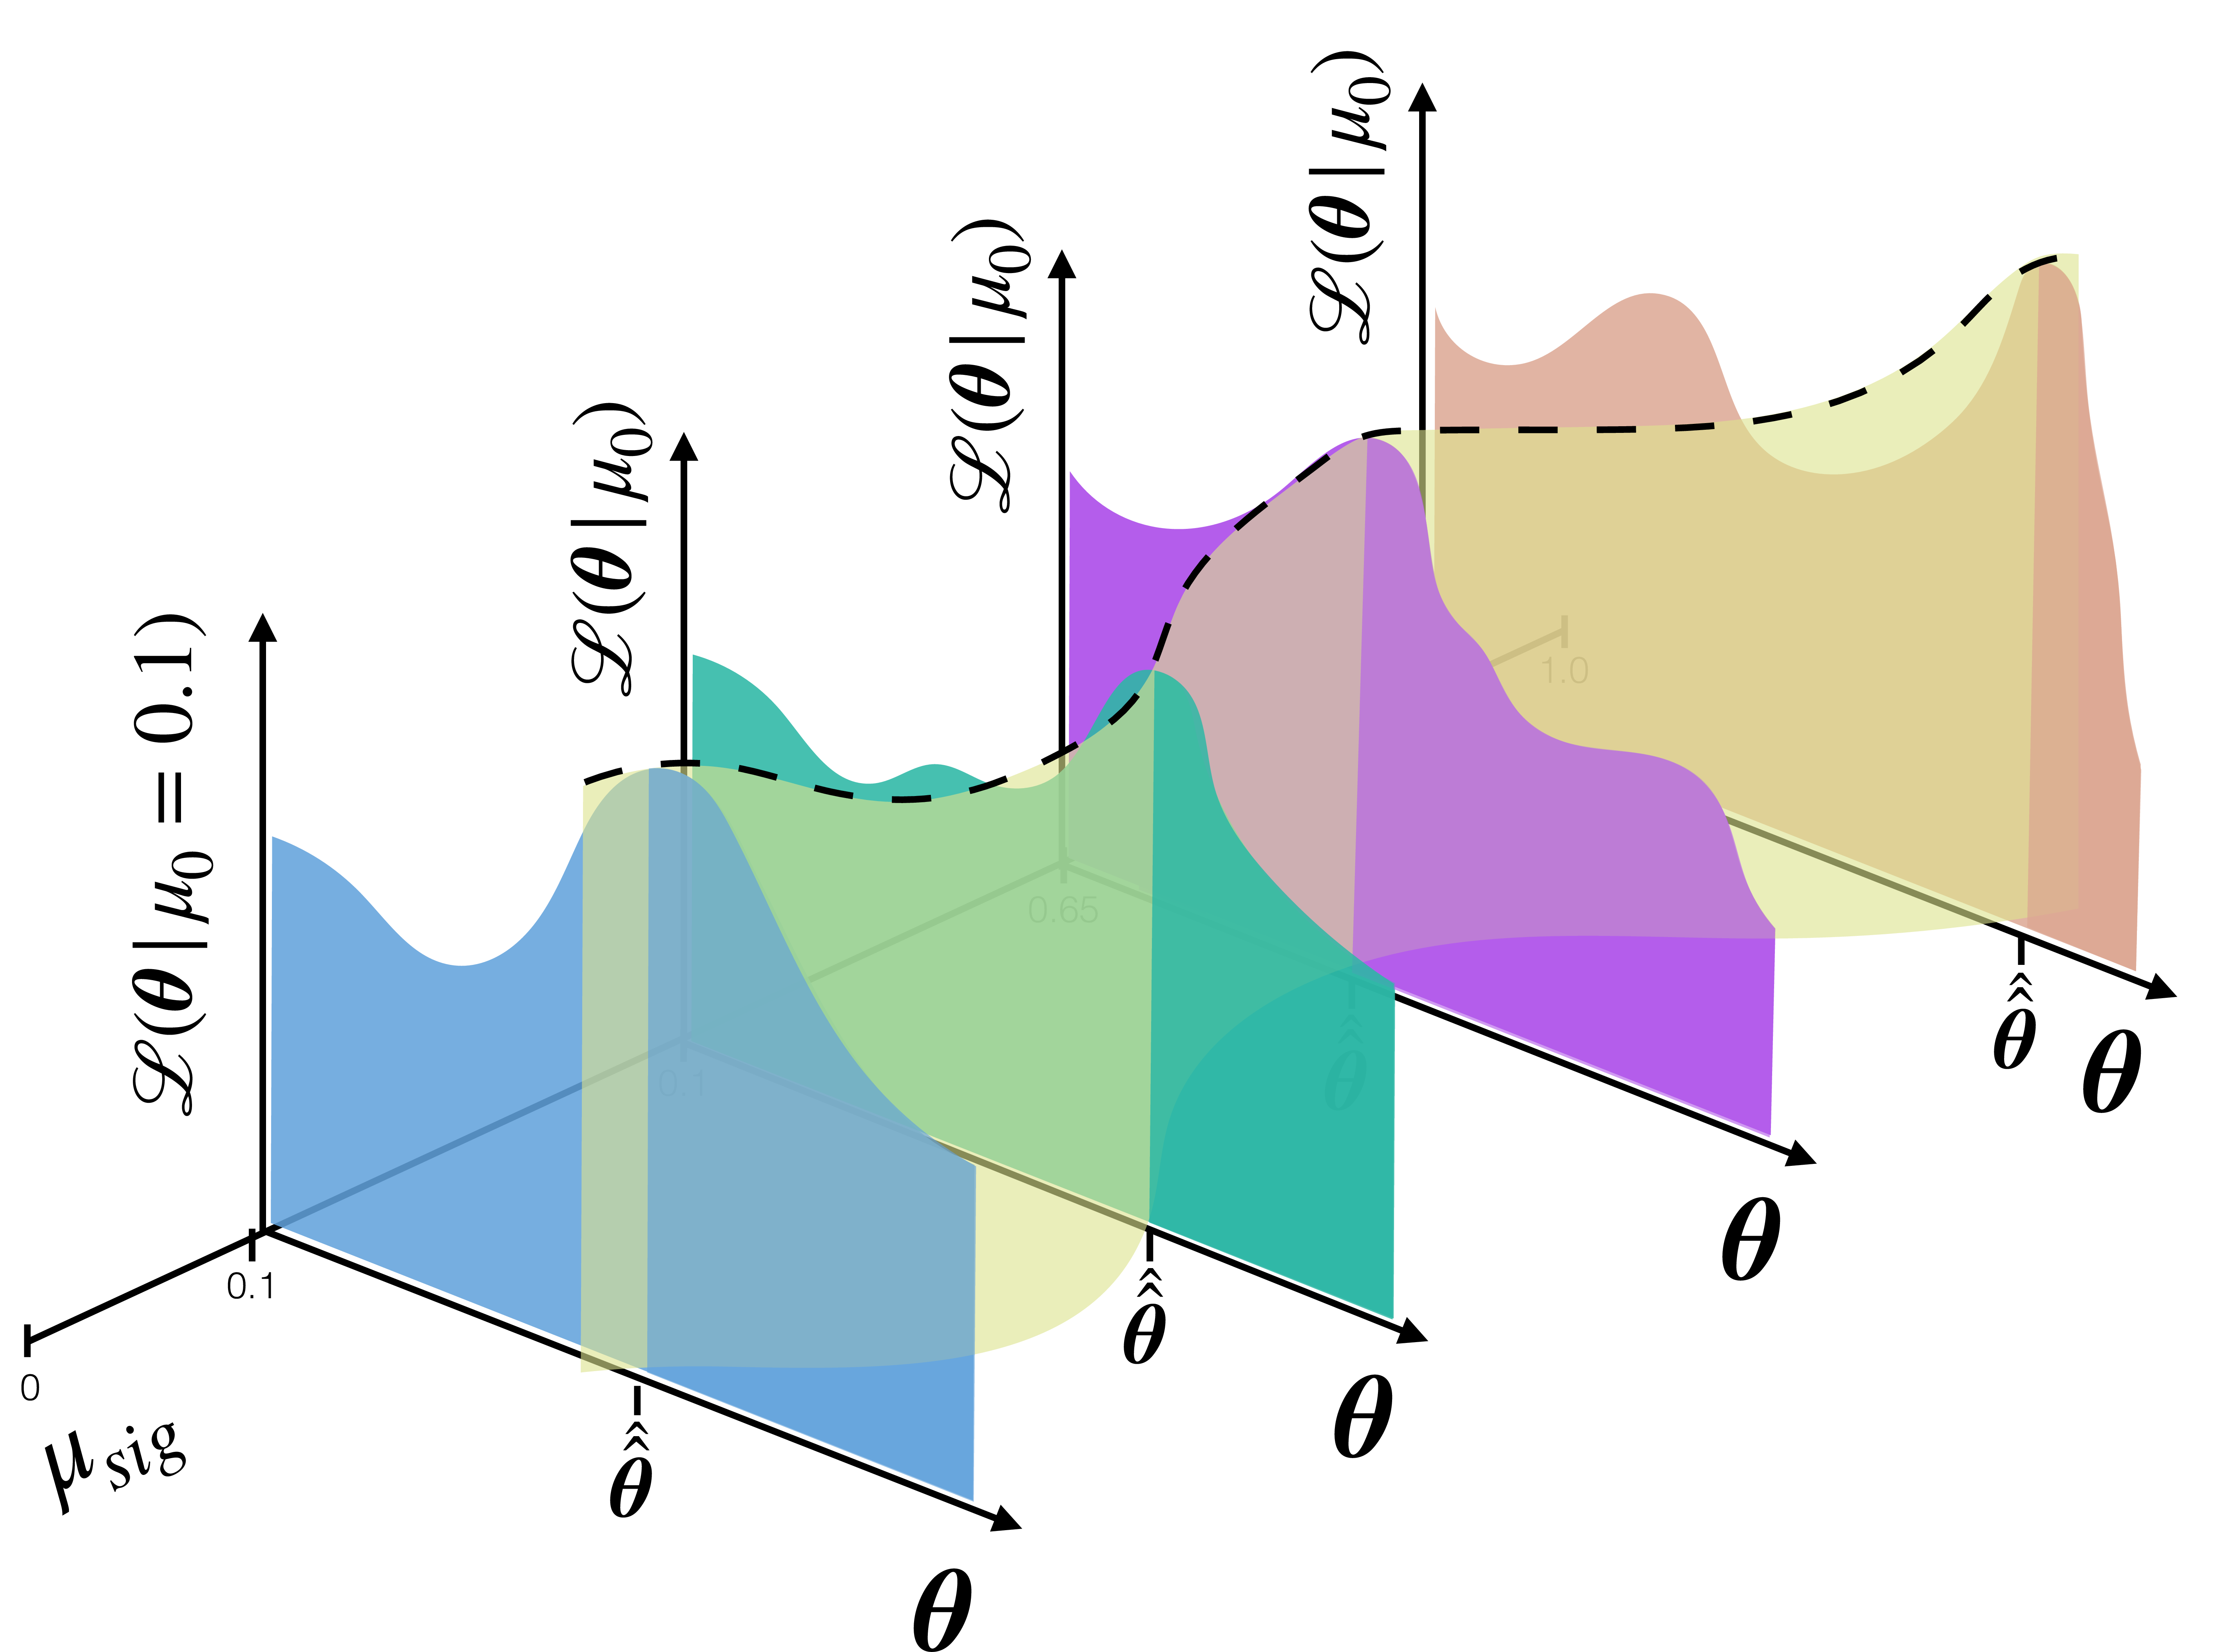
\includegraphics[width=0.98\textwidth]{figs/rpvthreel/LikelihoodProfileCartoon.png}
  \end{center}
  \caption[Cartoon of the Profile Likelihood.]
          {Cartoon of the Profile Likelihood.}
          \label{fig:ProfileLikelihood}
\end{figure}

\subsection{The Statistical Test: Profile Log Likelihood Ratio Test}
\label{sec:stats:LikelihoodRatio}
In order to then assess the goodness of fit of two competing statistical models, i.e. some BSM signal models against the SM, the profile log likelihood ratio test is employed. 
Whereby the Neyman–Pearson lemma, the likelihood-ratio test has the highest power among all statistical test competitors for comparing two models, each of which has no unknown parameters.
In general, for a statistical model $\Theta$ with subset $\Theta_{0}$ the specified parameter set $\boldsymbol\theta_{0}$ in $\Theta_{0}$ defines the null hypothesis $H_{0}$.
The alternative hypothesis $\boldsymbol\theta_{1}$ then exists in the compliment parameter space $\Theta_{0}^{c}$.
The likelihood ratio test is then given by Equation \ref{eq:LR}
%\begin{equation}
%    \lambda = \frac{\mathcal{L}(\boldsymbol\theta_{0}|k)}{\mathcal{L}(\b%oldsymbol\theta_{1}|k)}
%    \label{eq:LR} 
%\end{equation}
%where often the natural log is taken
\begin{equation}
    q = -2\ln\left[ \frac{\mathcal{L}(\boldsymbol\theta_{0}|k)}{\mathcal{L}(\boldsymbol\theta_{1}|k)} \right]
    \label{eq:LR}
\end{equation}
%The likelihood-ratio test then provides the following decision rule:
%\begin{equation*}
%  \begin{split}
%    &\textrm{if } q > c, \textrm{ do not reject } H_{0}; \\
%    &\textrm{if } q < c, \textrm{ reject } H_{0}; \\
%    &\textrm{Reject with probability } q \textrm{ if } q = c.
%  \end{split}
%\end{equation*}
The profile log likelihood ratio test can then be written as:
\begin{equation}
    q_{\mu_{sig}} = -2\ln\left[ \frac{\mathcal{L}(\mu_{sig}, \hat{\vphantom{\rule{1pt}{0.1ex}}\hat{\boldsymbol{\theta}}})}{\mathcal{L}(\hat{\mu}_{sig},\hat{\vphantom{\rule{1pt}{0.1ex}}\hat{\boldsymbol{\theta}}})} \right]
    \label{eq:pLR}
\end{equation}
Where $\hat{\mu}_{sig}, \hat{\vphantom{\rule{1pt}{0.1ex}}\hat{\boldsymbol{\theta}}}$  maximize the likelihood function and $\hat{\vphantom{\rule{1pt}{0.1ex}}\hat{\boldsymbol{\theta}}}$ maximize the likelihood for the specific, fixed value of the signal strength as was detailed in the previous Section~\ref{sec:stats:ProfileLiklihood}.
In this way a distribution of the test statistic $q$ can be built up by scanning over $\hat{\mu}_{sig},\hat{\vphantom{\rule{1pt}{0.1ex}}\hat{\boldsymbol{\theta}}}$ values to which a significance, i.e. the $p$-value can be attained.  
Figure \ref{fig:teststat} illustrates the distribution of $q_{\mu_{sig}}$ and it's relation to the $p$-value. 
\begin{figure}[tbp]
  \begin{center}
    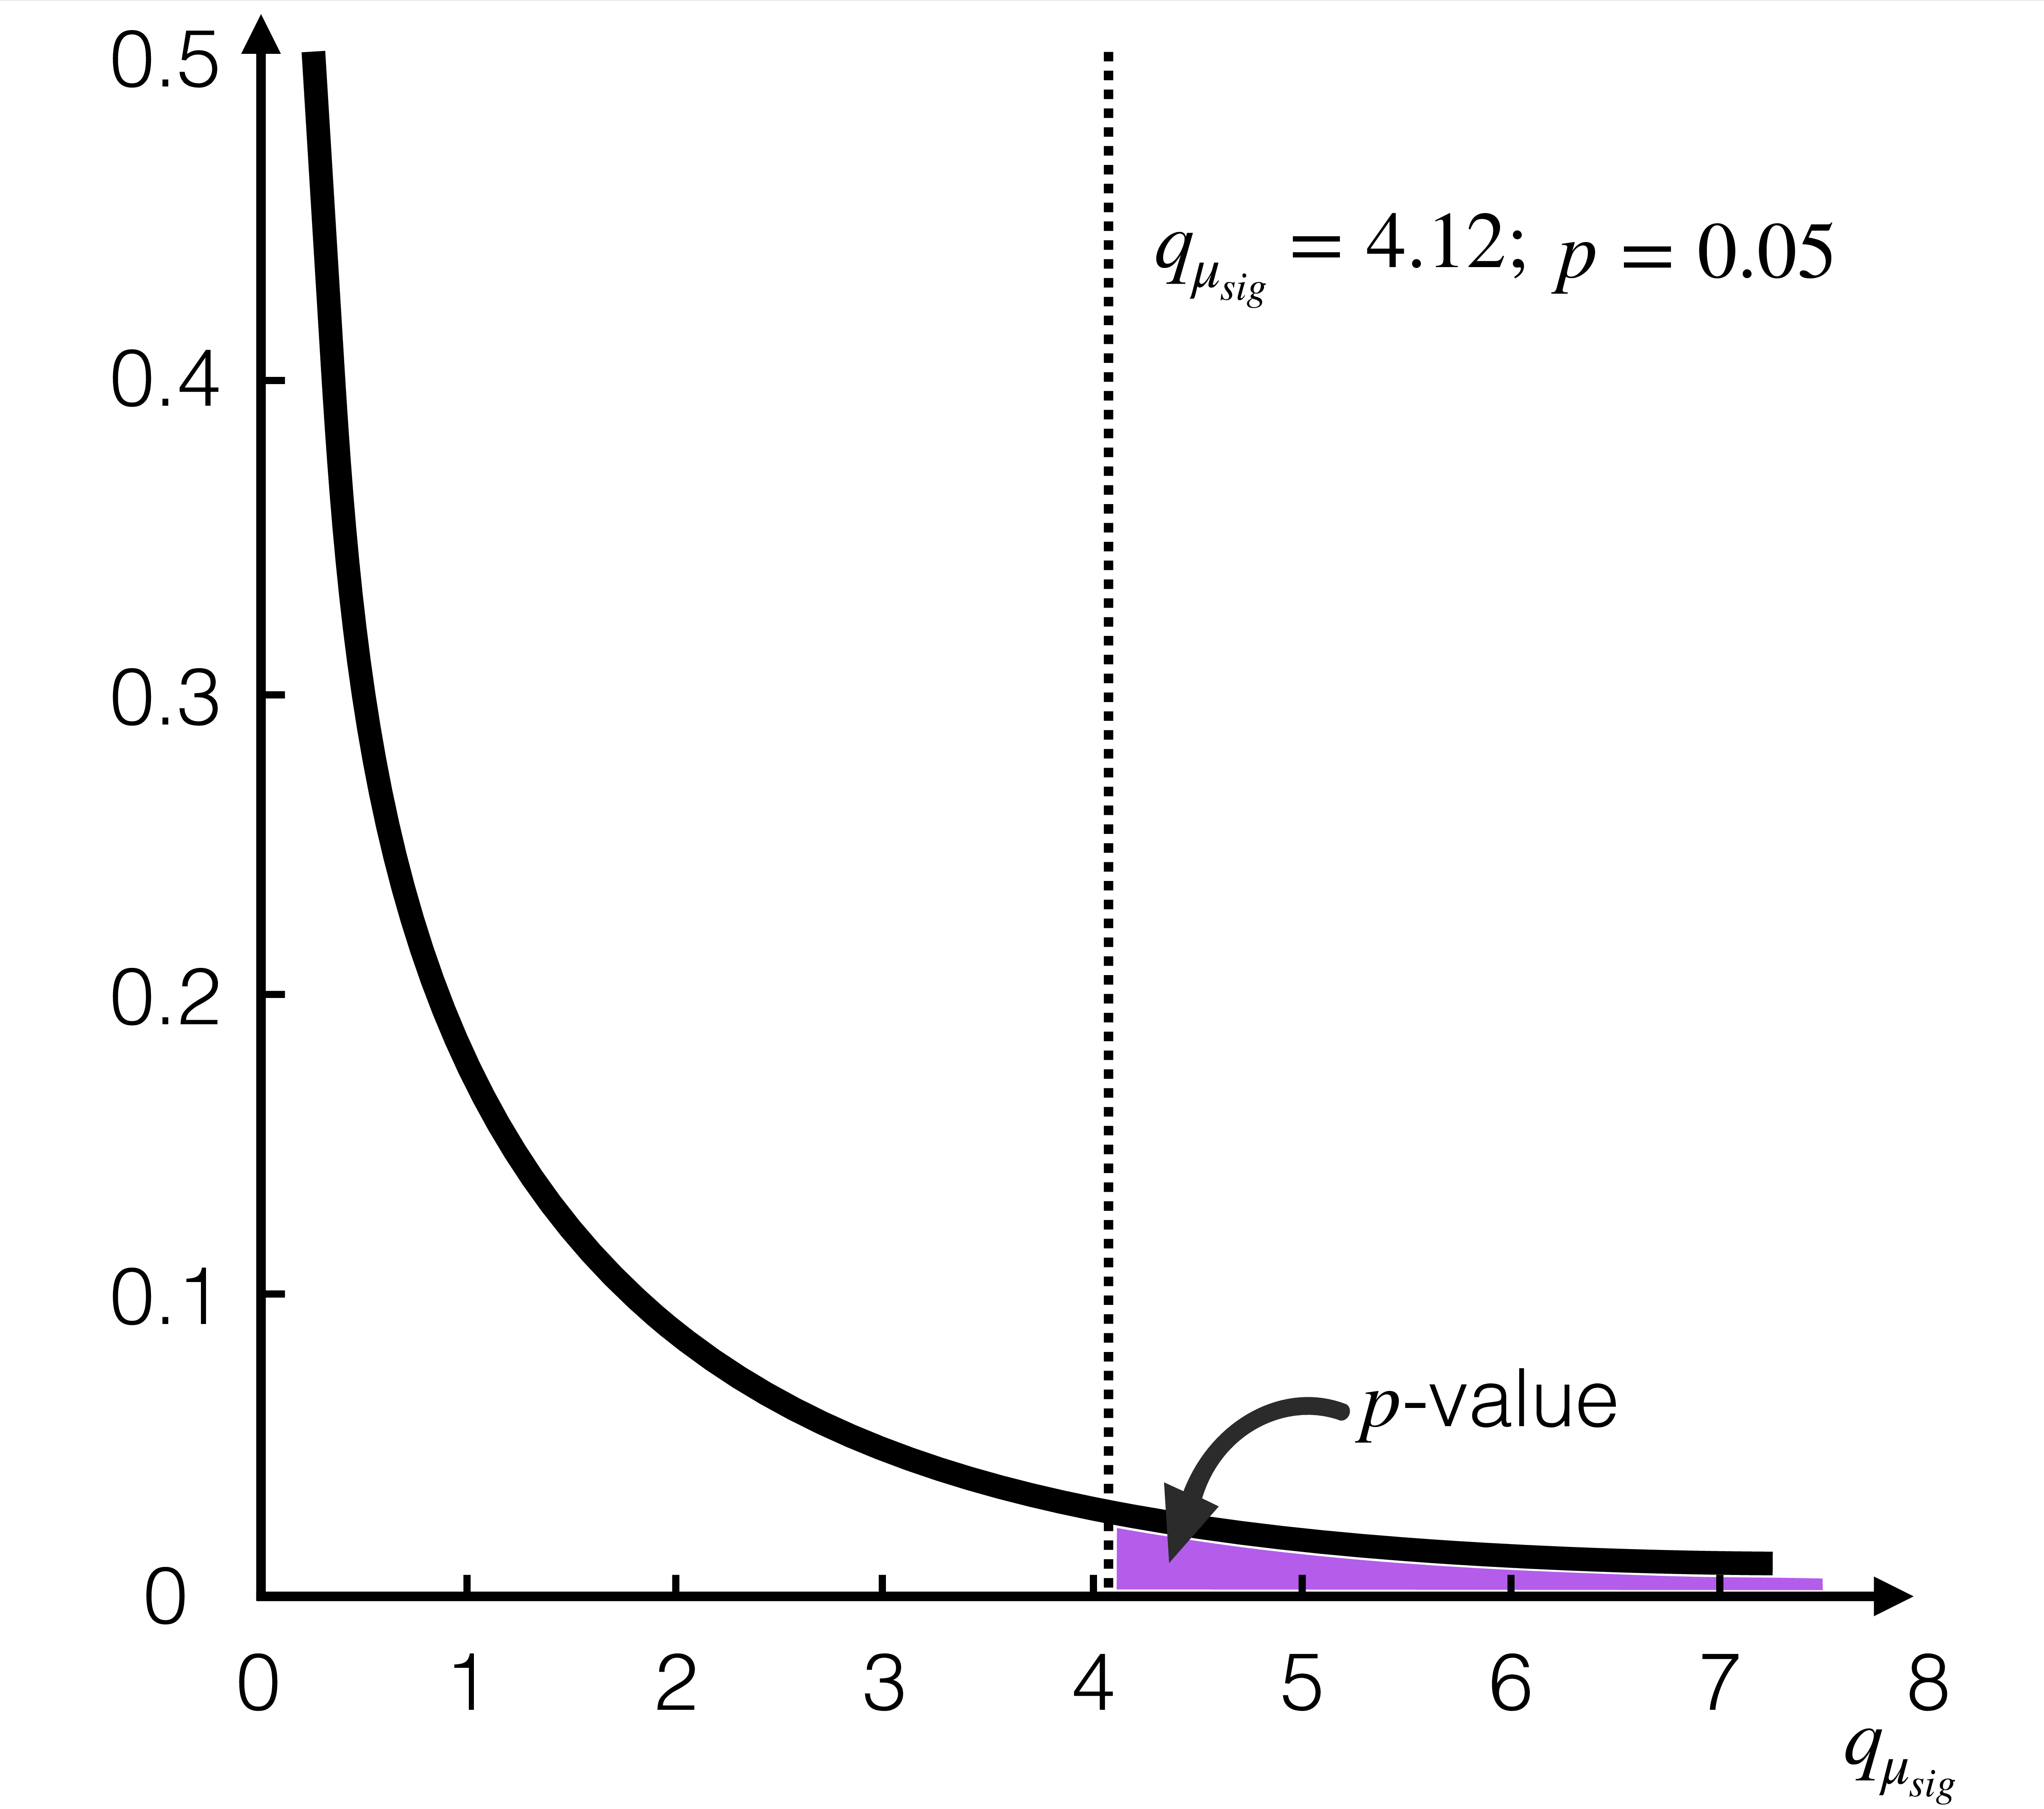
\includegraphics[width=0.98\textwidth]{figs/rpvthreel/teststatdistpvalue.png}
  \end{center}
  \caption[Illustration of a test statistic distribution and an observed $q_{\mu_{sig}}$ with corresponding $p$-value.]
          {Illustration of a test statistic distribution and an observed $q_{\mu_{sig}}$ with corresponding $p$-value as the purple area.}
          \label{fig:teststat}
\end{figure}


\subsection{The Asymptotic Regime}
The profile likelihood is constructed in two ways in this analysis.
First, the \emph{asymptotic method} is employed in the regime of a relatively large number of statistics, typically for event counts $O(10)$ and larger, Wilk's theorem states that the distribution of the test statistic, $q$, asymptotically approaches the chi-squared distribution under the null hypothesis~\cite{Wilks:1938dza}. 
The logic follows that asymptotically, $\mathcal{L}(\boldsymbol\theta|k)$ is gaussian, and then
\begin{equation*}
  \mathcal{L} = \exp{\left[-\frac{1}{2}\left(\frac{\mu-\hat{\mu}}{\sigma_{\mu}}\right)^{2}\right]} \implies q_{\mu_{0}} = \left(\frac{\mu_{0}-\hat{\mu}}{\sigma_{\mu}}\right)^2, \hspace{0.3cm} \hat{\mu}\sim G(\mu_{0}, \sigma_{\mu}) \implies q_{0}\sim\chi^{2}(n_{dof}=1)
  \label{eq:asymptotic}
\end{equation*}
In this asymptotic regime $\mathcal{L}$ becomes independent of the values of the auxiliary measurements. As a result, when using this procedure, the p-value obtained from the hypothesis test is robust, and generally will not undercover.

\subsection{Building the Profile Likelihood: Pseudo-Experiments}
In the regime where the number of events is fewer than $O(10)$, and the distributions are not assumed to take on their asymptotic form, the profile likelihood must be constructed using Monte Carlo methods.
In this “toy Monte Carlo” approach one generates pseudo-experiments in which the number of events in each channel $i$, the values of the discriminating variable, \mZl, for each of those events, and the auxiliary measurements (global observables), $\boldsymbol\theta_{0}$, are all randomized according to $\mathcal{L}(\boldsymbol\theta|k)$ (Eq.~\ref{eq:statmodel}).
%We denote the resulting data Dtoy and global observables Gtoy.
By doing this many times one can build an ensemble of pseudo-experiments (generating a test statistic distribution) and evaluate the necessary integrals.
%The choice of $\mu_{sig}$ is straight forward: typically $\mu_{sig}$=0 and $\mu_{sig}$=1, but choice of $\boldsymbol\theta$ is less clear

\subsection{Significance and the $\mathrm{CL_{s}}$ Method}
\label{sec:stats:CLs}
In the event that no significant excess is seen above the SM, limits are set on new physics. 
The prescription used to set these limits is known as the \emph{$CL_S$ Method}.
Given the test statistic distribution $f(\tilde q_{\mu} |\mu,\hat{\vphantom{\rule{1pt}{0.1ex}}\hat{\boldsymbol{\theta}}}(\mu,\textrm{obs}))$, determined from either pseudo-experiments or asymptotics, both described in previous sections, the following $p$-value is used to quantify consistency with the hypothesis of a signal strength of $\mu$ ($\mu_{sig}$).
\begin{equation}
    p_{\mu} =\int_{\tilde q_{\mu,\textrm{obs}}}^{\infty} f(\tilde q_{\mu} |\mu,\hat{\vphantom{\rule{1pt}{0.1ex}}\hat{\boldsymbol{\theta}}}(\mu,\textrm{obs}))~d\tilde q_{\mu}
\end{equation}
Now a standard 95\% confidence-level, one-sided frequentist confidence interval (upper limit) is obtained by solving for $p'_{\mu_{up}}$ = 5\%.
For downward fluctuations the upper limit of the confidence interval can be
arbitrarily small, though it will always include $\mu$ = 0.
This feature is considered undesirable since a physicist would not claim sensitivity to an arbitrarily small signal rate.
The feature was the motivation for the modified frequentist method called CLs and the alternative approach called power constrained limits.
To calculate the CLs upper limit, we define $p'_{\mu}$ as a ratio of $p$-values
\begin{equation}
    p'_{\mu} = \frac{p_{\mu}}{1-p_{b}}
\end{equation}
where $p_{b}$ is the $p$-value derived from the same test statistic under the background-only hypothesis
\begin{equation}
    p_{b} = 1 - \int_{\tilde q_{\mu,\textrm{obs}}}^{\infty} f(\tilde q_{\mu} |0,\hat{\vphantom{\rule{1pt}{0.1ex}}\hat{\boldsymbol{\theta}}}(\mu=0,\textrm{obs}))~d\tilde q_{\mu}
\end{equation}
The CLs upper-limit on $\mu$ is denoted $\mu_{up}$ and obtained by solving for $p'_{\mu_{up}}$ = 5\%.
It is worth noting that while confidence intervals produced with the ``CLs'' method over cover, a value of $\mu$ is regarded as excluded at the 95\% confidence level if $\mu<\mu_{up}$.
The amount of over coverage is not immediately obvious; however, for small values of $\mu$ the coverage approaches 100\% and for large values of $\mu$ the coverage is near the nominal 95\% (due to $\langle p_{b} \rangle$ $\approx$ 0).
For the purposes discovery one is interested in compatibility of the data with the background-only
hypothesis.Statistically, a discovery corresponds to rejecting the background-only hypothesis.
This compatibility is based on the following p-value
\begin{equation}
    p_{0} =\int_{\tilde q_{0,\textrm{obs}}}^{\infty} f(\tilde q_{0} |0,\hat{\vphantom{\rule{1pt}{0.1ex}}\hat{\boldsymbol{\theta}}}(\mu=0,\textrm{obs}))~d\tilde q_{0}
\end{equation}

This $p$-value is also based on the background-only hypothesis, but the test statistic $\tilde q_{0}$ is suited for testing the background-only while the test statistic $\tilde q_{\mu}$ in Eq. 59 is suited for testing a hypothesis with signal.
It is customary to convert the background-only $p$-value into the quantile (or ``sigma'') of a unit Gaussian.
This conversion is purely conventional and makes no assumption that the test statistic $q_{0}$ is Gaussian distributed.
The conversion is defined as:
\begin{equation}
    Z = \Phi^{-1}(1-p_{0})
\end{equation}
Where $\Phi^{-1}$ is the inverse of the cumulative distribution for a unit Gaussian.
One says the significance of the result is $Z\sigma$ and the standard discovery convention is 5$\sigma$, corresponding to $p_{0}$ = 2.87$\times 10^{-7}$.
Most of this section was taken directly from~\cite{Cranmer:2014lly}.

%For each signal model, a simultaneous fit is performed to the control regions and the signal regions, fitting to the number of events passing each selection criteria. 
%At any given point in the exclusion interval (the mass region with
%$CL_{s}(m{\chono}) \leq$ 5\%) the probability of having falsely excluded a true Higgs at that mH is less than 5\%. 
%The smaller the value of CLs($m_{H}$) the more confident we can be that we have not missed observing a Higgs with mass m